\section{Simulation}



PARNTR provides a common framework for embodied robotic agents to interact within a digital indoor environment to solve a task.  Two robotic agents are simulated within the environment: (1) a humanoid robot and (2) a Boston Dynamics Spot robot.  It should be noted that the spot robot and the humanoid robot have different capabilities.  The humanoid robot can perform all the actions of the Spot robot, but has additional capabilities.

\textbf{Spot Robot Capabilities:}
\begin{itemize}
      \item \textbf{Close:}
            Used for closing an articulated entity. You must provide the name of the furniture you want to close.
      \item \textbf{Explore:}
            Search a specific room by visiting various receptacles or furniture in that room. The input to the skill is the EXACT name of the room to be visited. Use the room names provided in the house description. This tool exhaustively explores the specified room.
      \item \textbf{Navigate:}
            Used for navigating to an entity. You must provide the name of the entity you want to navigate to.
      \item \textbf{Open:}
            Used for opening an articulated entity. You must provide the name of the furniture you want to open.
      \item \textbf{Pick:}
            Used for picking up an object. You must provide the name of the object to be picked. The agent cannot hold more than one object at a time.
      \item \textbf{Place:}
            Used for placing an object on a target location. You need to provide the name of the object to be placed, the name of the furniture where it should be placed, spatial relation ("on" or "within") describing the relation between the object and furniture. The object to be placed must already be held by the agent (i.e. picked previously).
      \item \textbf{Rearrange:}
            Used for moving an object from its current location to the target location. You need to provide the name of the object to be moved, the name of the furniture where it should be moved, spatial relation ("on" or "within") describing the relation between the object and furniture. This will automatically pick the specified object and move to the target furniture and attempt to place it.
      \item \textbf{Wait:}
            Used to make agent stay idle for some time.
\end{itemize}



\textbf{Humanoid Robot Capabilities:} The humanoid robot has all the capabilities of the Spot robot and a few additional capabilities:

\begin{itemize}
      \item \textbf{Clean:}
            Used for cleaning an object. You need to provide the name of the object to clean.
      \item \textbf{Fill:}
            Used for filling an object. You need to provide the name of the object to fill.
      \item \textbf{Pour:}
            Used for pouring from one container to another. This skill will pour into the specified container from whichever container is currently held by the agent.
      \item \textbf{PowerOff:}
            Used for turning off a powered object. You need to provide the name of the object to be turned off.
      \item \textbf{PowerOn:}
            Used for turning on a powered object. You need to provide the name of the object to be turned on.
\end{itemize}

When designing our experiments we focused on two key areas: (1) \textit{centralized planning} versus \textit{decentralized planning} and (2) \textit{fully observable} versus \textit{partially observable}.  We wanted to understand how well frontier LLMs could correctly plan out their actions in randomized indoor scenes with different levels of observability.  We were not necessarily concerned about the physical interactions (i.e. motor controls) of the robots, thus we abstracted away motor controls.  A robot could perform an action on an object as long as it was close to the object.

\begin{itemize}
      \item \textbf{Centralized vs Decentralized Planning:}
            In centralized planning, a single LLM decides actions for both agents, with complete information about both agent's states; effectively removing any need for coordination between the agents. In decentralized planning, each agent is controlled by a different LLM, and each LLM needs to reason about the other agent's actions. See Figure~\ref{fig:central_vs_decentral}.
      \item \textbf{Partial vs Full Observability:}
            In partially observed environments the planner knows the house's layout, but objects are hidden.  The location of hidden objects can only be discovered using exploration actions. In fully observed environments room layout and all object locations are visible.
\end{itemize}

Iterating over all possible combinations, we have Table-\ref{tab:experiment_design}:

\begin{table}[ht]
      \centering
      \fontfamily{ppl}\selectfont
      \begin{tabular}{lll}
            \toprule
            Planner       & Observability & Difficulty \\
            \midrule
            Centralized   & Full          & Easy       \\
            Centralized   & Partial       & Moderate   \\
            Decentralized & Full          & Moderate   \\
            Decentralized & Partial       & Hard       \\
            \bottomrule
      \end{tabular}
      \caption{Design matrix for setting up experiments.}
      \label{tab:experiment_design}
\end{table}

\begin{figure*}
      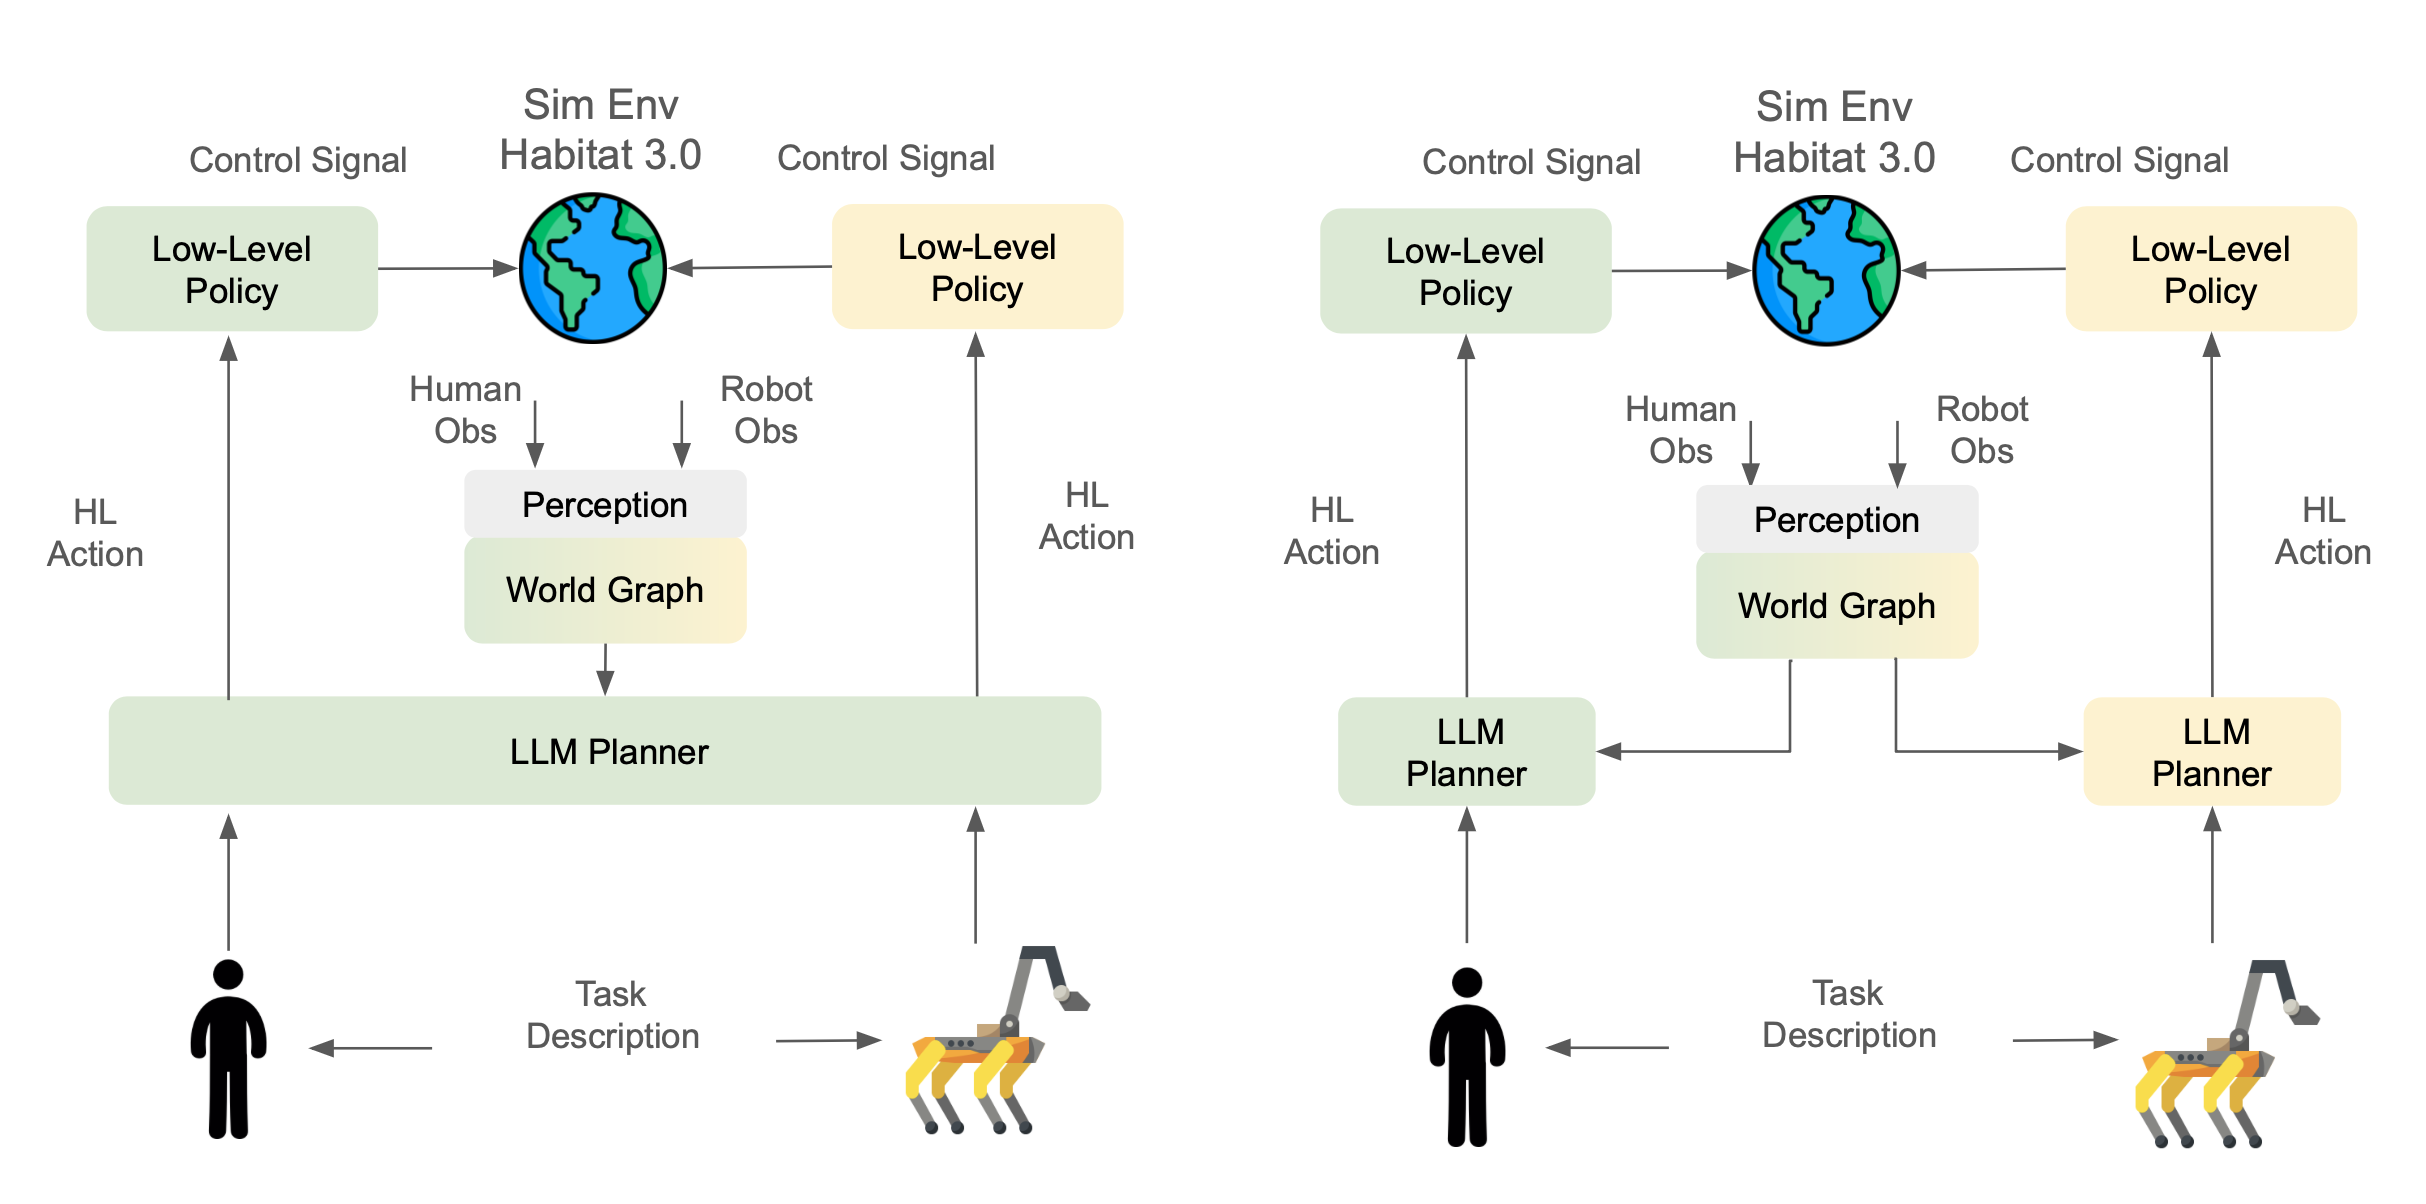
\includegraphics[width=0.85\paperwidth]{agent-architecture.png}
      \caption{\textbf{Centralized vs Decentralized Planning:} In the centralized planner, one planner controls the actions of both agents.  The actions are sent to a low-level policy which mechanically performs the actions.  These actions are then updated within the simulator (Habitat 3.0) and outputs a new state which is then observed individually by each agent.  The observations update a shared world graph which is fed back into the centralized planner repeating the process.  The decentralized planner in contrast has separate planners for each agent.  In decentralized planning the agents have individual observations which are used to update a non-shared world graph.  The figure was sourced from PARTNR\cite{chang2024partnrbenchmarkplanningreasoning}.}
      \label{fig:central_vs_decentral}
\end{figure*}

Centralized planning is considered an easier task than decentralized planning.  Full observability is considered easier than partial observability.  For each experimental design configuration, we provide a difficulty estimate based on the combination of different parameters.  From an information standpoint, the decentralized planner can be thought of partial observability because each planner must perform planning without knowing what the other planner is doing.  The difficult assessment is really a ranking of how much information the planner has to perform its planning cycle given the limited information it has access to.

PARTNR provides a way for LLMs to interact with its environment purely using text.  This is an oversimplification because real robotics would use a live camera feed for scene perception.  For the purposes of our study, we were focused on planning and coordination of frontier LLMs in embodied robotics; camera perception was not our focus, so we decided to use a text based interactive environment.

At the start of an episode, the agents would be randomly placed somewhere in the environment.  Rooms and objects are randomized.  PARTNR would then generate a task in natural language for the indoor simulations.  Consider Example~\ref{ex:example_task} where the environment is partially observable, the agent is tasked with finding the sushi mat and move it to the living room table.  The sushi mat is not directly observed meaning the agent must explore the indoor environment to find the sushi mat.  After finding the sushi mat, it must navigate to it, pick it up, navigate to the living room table, and then place it on the living room table.

\begin{Example}{Example Task \& State of Knowledge}{Partially Observable}

      \textbf{Task:} Move the \textbf{\textcolor{brown}{sushi mat}} from the \textbf{\textcolor{red}{kitchen counter}} to the  \textbf{\textcolor{blue}{living room table}}.

      \medskip
      \textbf{State Information:}
      \begin{itemize}
            \item \textbf{living\_room\_1:}
                  \begin{itemize}
                        \item floor\_living\_room\_1
                        \item \textbf{\textcolor{blue}{table\_14}}
                        \item \textbf{\textcolor{blue}{table\_15}}
                        \item couch\_23
                        \item chair\_32
                  \end{itemize}
            \item \textbf{bathroom\_1:}
                  \begin{itemize}
                        \item floor\_bathroom\_1
                        \item toilet\_30
                  \end{itemize}
            \item \textbf{kitchen\_1:}
                  \begin{itemize}
                        \item stool\_18
                        \item stool\_19
                        \item \textbf{\textcolor{red}{counter\_34}}
                        \item cabinet\_35
                        \item cabinet\_41
                  \end{itemize}
            \item \textbf{dining\_room\_1:}
                  \begin{itemize}
                        \item floor\_dining\_room\_1
                        \item chair\_10
                        \item chair\_11
                        \item chair\_12
                        \item chair\_13
                        \item table\_21
                  \end{itemize}
      \end{itemize}
      \medskip



\end{Example}\label{ex:example_task}

\begin{Example}{Example Plan}{Partially Observable}
      \textbf{Example Planning:}
      \begin{enumerate}
            \item Explore kitchen
            \item Navigate to kitchen counter\_34
            \item Pickup sushi\_mat
            \item Navigate to living\_room\_1
            \item Put sushi\_mat on table\_14
      \end{enumerate}
\end{Example}\label{ex:example_plan}